\section{Suggesting Changes In View(s Types)}
\label{sec:Suggestion}

Figure \ref{fig:Suggestion} depicts a \metamodel that captures the
required elements for helping methodologists improve their \viewtype designs,
by suggesting possible ways to reflect evolution changes inside \viewtypes.
In the following, we assume that a methodologist is working on a \metamodel
under evolution \textsf{MM}, that is linked to a set $\mathsf{VT}$ of viewtypes
(i.e. $\mathsf{VT} = (\mathsf{VT}_\mathsf{i})_{\mathsf{i}\in [1..n]}$). Note that in the discussion above, when we discuss
\textsf{MM}'s (meta-)elements, we consider \textsf{MM} as a \emph{model}
conforming to a particular meta-\metamodel (such as \textsc{Mof} \cite{TR:OMG-MOF:2016}):
we therefore discuss changes on \textsf{MM}'s packages, classes (e.g. 
\textsf{FSM} or \textsf{State} in our example) and their structural features
(such as the attribute \textsf{name} or the reference \textsf{src}).

A \textsf{Suggestion} is the core element of our approach, and contains three 
parts:
\begin{enumerate}
    \item A change \textsf{Operator}, detailed in Figure \ref{fig:Operator}, capturing the nature of
alterations operated on \textsf{MM}'s meta-elements; 
    \item A \textsf{Relation}, providing traceability links between \textsf{MM} 
		and \textsf{VT}: for each meta-element in \textsf{MM} subject to a 
		change by an \textsf{Operator}, a \textsf{Relation} identifies which 
		meta-elements in \textsf{VT} may be affected;
    \item A \textsf{Recommendation}, detailing possible actions a methodologist 
		may perform to realign \textsf{VT} after a change. 
		\item Some \textsf{Condition}s providing additional informations on the
		applicability of \textsf{Operator}s, as well as domain-specific knowledge.
		\MA{For now, I still don't see where these would be helpful in our example.
		We may still discuss that in general in the Discussion Section, but in that
		case, we should remove it from the \textsf{Suggestion} metamodel!}
\end{enumerate}

Note that a \textsf{Suggestion} may 
associate \emph{no} \textsf{Recommendation}s, in case an \textsf{Operator} has no
impact on \viewtypes; or \emph{several} \textsf{Recommendation}s for the same 
\textsf{Operator}, depending on the \textsf{Operator}'s complexity, and how 
many \viewtypes are concerned by the \textsf{Operator}.

The rest of this Section details each part in a \textsf{Suggestion}; a summary
is presented in Table \ref{tab:suggestions}.

\subsection{Change}
\label{sec:Suggestion:Change}

\begin{figure}[t]
    \centering
    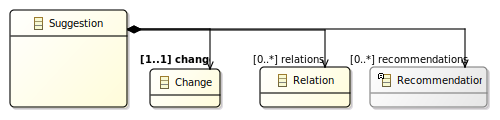
\includegraphics[width=\columnwidth]{images/Suggestion.pdf}
    \caption{A \textsf{Suggestion} holds for a single \textsf{Change} linked to 
		elements in a View Type through \textsf{Relation}s, and consists of a set of \textsf{Recommendation}s.}
    \label{fig:Suggestion}
\end{figure}

A \textsf{Change} refers to an \textsf{Operator} that may be parameterised with 
extra data, and contains contextual information (in \textsf{ApplicationPattern}\LC{what is meant by this? ApplicationPattern is not visible in any Figure, and Googling it, is not immediately clear which if any specific design pattern it refers to, if that's what's intended}). 
Change \textsf{Operator}s may target \emph{any} instantiable \metamodel element, 
thus referring to the class \textsf{NamedElement} in \textsc{Mof}. Note that we 
will distinguish between \emph{primitive} and \emph{complex} \textsf{Operator}s,
depending on the number of such \metamodel elements an \textsf{Operator} acts on.

Since \viewtypes are structurally \metamodels, we reviewed the literature to
identify relevant change \textsf{Operator}s. In our work, we integrate all 27 \textit{primitive} and seven of the 34 \textit{complex} operators in the change catalogue proposed by Herrmannsdoerfer et al.~\cite{herrmannsdoerfer_extensive_2011}.
These seven were selected because they constitute 72\% of all complex changes appearing in a large case study (cf. \cite{khelladi_detecting_2015}). 

\textsf{Operator}s are enriched with a \emph{severity}: \emph{Major}
(abbreviated as \textsf{M}), \emph{miNor} (\textsf{N}) and \emph{Ignore} 
(\textsf{I}). 
When applied to a \metamodel, the \textsf{Operator}s in \textsf{I} have no effect
on the corresponding \viewtypes; \textsf{Operator}s that can break the relationship
between \textsf{MM }and its \viewtypes are categorised as \textsf{M}; the rest of the
\textsf{Operator}s are \textsf{N}, since they are not breaking and can enrich 
the \viewtypes with additional information.\LC{Idea I've applied to table, to save space/cognitive load on table: dropped the 'I' operator rows from the table completely; instead adding next sentence here:} The seven \textsf{Operator}s \textsf{Make/Drop Class Abstract}, \textsf{Make/Drop Attribute Identifier}, \textsf{Make/Switch Reference Composite}, and \textsf{Pull Property} are of type \textsf{I} and hence not included in Table~\ref{tab:suggestions} of suggestions per change operator.

\begin{figure}[t]
    \centering
    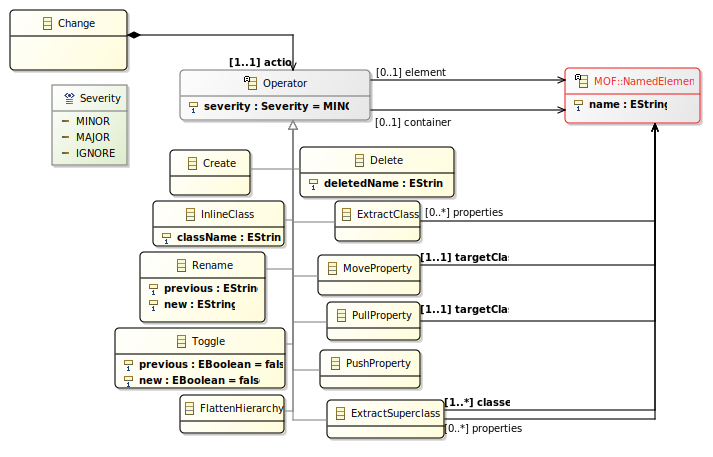
\includegraphics[width=\columnwidth]{Change.pdf}
    \caption{Possible \textsf{Operator}s for \metamodel evolution.}
    \label{fig:Change}
\end{figure}

The evolution steps of Figure \ref{fig:FSM} make use of different \textsf{Operator}s.
\begin{itemize}
	\item In Step 1 (depicted from Figure \ref{fig:FSM:Init} to \ref{fig:FSM:Relevant}),
	the following sequence of \textsf{Operator}s is applied:
	$$\langle \mathsf{PushProperty} \cdot \mathsf{Rename} \cdot \mathsf{Rename} \rangle$$
	First, \textsf{PushProperty} pushes down $\mathsf{Named} \squaredots \mathsf{name}$
	(i.e. pushes down the \textsf{element} \textsf{name} in the \textsf{container}
	\textsf{Named})
	into each subclass (namely, \textsf{FSM}, \textsf{State} and \textsf{Transition});
	then \textsf{Rename} is applied to the \textsf{element} \textsf{name}, 
	located respectively in \textsf{container}s $\mathsf{FSM}$ and 
	$\mathsf{Transition}$, thus obtaining the result of Figure \ref{fig:FSM:Relevant}.
	
	\item Step 2 only consists of the following \textsf{Operator} sequence:
	$$\langle \mathsf{Create} \cdot \mathsf{Create} \cdot \mathsf{Create} \rangle$$
	where each \textsf{Operator} adds a new Attribute \textsf{element} in 
	\textsf{container} \textsf{Transition}, ending up in the situation of
	Figure \ref{fig:FSM:Guard}.
	
	\item Step 3 requires a longer sequence of \textsf{Operator}s, since it creates
	a new class hieararchy under \textsf{Expression}. However, this sequence may
	start with the following:
	$$\langle \mathsf{Delete}^3 \cdot \mathsf{Create}^2 \cdot \ldots \rangle$$
	The initial \textsf{Delete}s undo the \textsf{Create} operations of Step 2
	(thus, referring to the same \textsf{element}s and \textsf{container}); and
	the two following \textsf{Create}s create the new \textsf{Expression} class
	(with the default package as a \textsf{container}) and the \textsf{guard}
	reference (with \textsf{Transition} as a \textsf{container}).
\end{itemize}
With these examples, we immediately notice that some \textsf{Operator}s
in a \textsf{Change} sequence may depend on previous ones (e.g. \textsf{Rename}
in Step 1 should only be performed after \textsf{PushProperty}); while others
may freely commute (e.g. the \textsf{Create} in Step 2 may be performed in any 
order).
\subsection{Relations}
\label{sec:Suggestion:Relation}


\subsection{Recommendation}
\label{sec:Suggestion:Recommendation}

Wheras an \textsf{Operator} concerns \textsf{MM}, a \textsf{Recommendation} 
describes an action a methodologist may perform on \textsf{VT} in order to
co-evolve \viewtypes. 
In our approach, we issue a \textsf{Recommendation} for each \viewtype element 
\textsf{impacted} by an \textsf{Operator}. We identified four kinds of \textsf{Action}s: 
\begin{itemize}
	\item a \textsf{DEL}ete action that a \viewtype element is no longer associated
	to an \textsf{MM} element, and thus may be deleted;
	\item an \textsf{ADD} action suggests to create a new element in the \viewtype
	to reflect a newly created \textsf{MM} element;
	\item an \textsf{UP}date action changes the (String) value of a \viewtype element;
	\item a \textsf{MOVE} action suggests to move a \viewtype element from a \textsf{src}
	(source) to \textsf{tgt} (target) container.
\end{itemize}
Note that each \textsf{Recommendation} action stores a \textsf{name} (which, for
\textsf{UP}date, corresponds to the new value, whereas \textsf{previous} 
indicates the original one), as well as its \textsf{container}, but also 
indicates the \textsf{type} of the \viewtype meta-element the 
\textsf{Recommendation} is performed on.

\autoref{tab:suggestions} provides the details of each \textsf{Recommendation} 
following the list of \textsf{Operator}s we identified in Sec. 
\ref{sec:Suggestion:Change} and commented in the next section.

\begin{figure}[t]
    \centering
    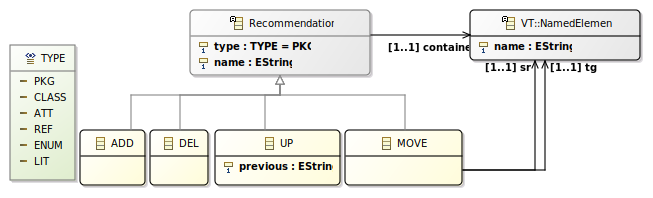
\includegraphics[width=\columnwidth]{Recommendation.pdf}
    \caption{\textsf{Recommendation}s actions suggested after a \textsf{Change}
    e.g. in Step 1, \textsf{ADD} Attribute \textsf{name} in \textsf{Transition} 
		\HM{i think it might be useful to include the word 'action' in the caption 
		as this figure is for that purpose. also do we have a sentence or so in the 
		running text explicitly mentioning about the difference between action and 
		operation?}
		\MA{Added ``action'' in caption. \textbf{What is an ``operation''}? Normally
		we only talk about \textsf{Operat\textbf{or}s!!!} If this is what you mean, yes: start of \S IV.C}}
    \label{fig:Recommendation}
\end{figure}
\subsection{Conditions}
\label{sec:Conditions}

